% 1. Какую систему Вы изучаете в Вашей диссертационной работе? Что является объектом исследования.
% 2. Каково назначение Вашей системы?
% 3. Какова цель исследования системы? Где она может быть использована?
% 4. Частью какой надсистемы является изучаемая система?
% 5. Из каких подсистем состоит система?
% 6. Какие задачи решают подсистемы в составе Вашей системы?
% 7. Сформулируйте кратко сценарий функционирования системы.

В качесте системы для исследования я обозначил структуру программного средства, предназначенного для интеграции в плагинную систему. Надсистемой является жизненный цикл ПО. Для выявления и описания подсистем мною проанализирована предметная область, сформулированы ограничения на компоненты системы и предложена формулировка ее описания в виде графовой модели. Модель состоит из следующих сущностей, к которым применены ограничения:
\begin{enumerate}
    \item сущности классифицированы:
    \begin{enumerate}
        \item включающая конкретный перечень плагинов поставка;
        \item пригодные для интеграции в плагинную систему плагины;
        \item распределенные по плагинам файлы исходного кода;
        \item функциональные зависимости между файлами исходного кода и плагинами;
        \item реализованные в файлах исходного кода требования.
    \end{enumerate}
    \item один файл исходного кода может реализовывать одно или несколько требований;
    \item одно требование может быть реализовано в одном или нескольких файлах исходного кода;
    \item один файл исходного кода не может быть включен в несколько плагинов;
    \item файлы исходного кода могут иметь зависимости друг на друга, в том числе и циклические;
    \item плагины так же имеют зависимости друг на друга: если в первый плагин включены файлы, зависящие от файлов, расположенных во втором плагине, то первый плагин зависим от второго;
    \item циклические зависимости между плагинами запрещены.
\end{enumerate}

Принципиальная схема приведена на рисунке \ref{fig:graph}.

\begin{figure}[H]
    \centering
    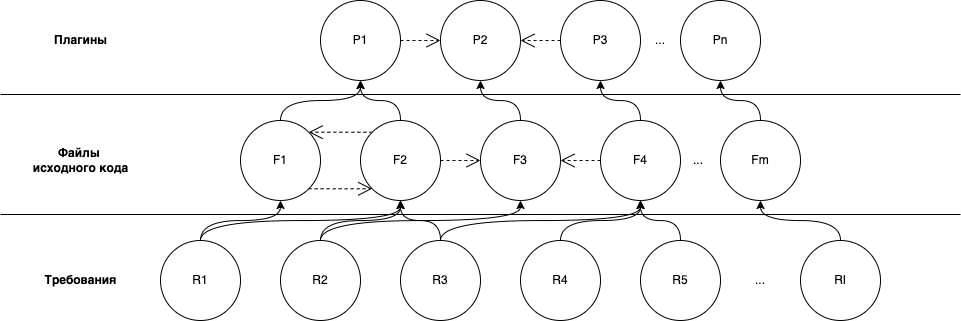
\includegraphics[width=1\textwidth]{graph}
    \caption{Система с приведенными подсистемами}
    \label{fig:graph}
\end{figure}

